\section{Основные уравнения}

\subsection{Определения теории фильтрации}

\par Основное явление, изучаемое в этой работе --- осаждение частиц на поверхности пористой среды. В ходе этого процесса частицы могут прикрепляться к пористому скелету, что влияет на течение жидкости и объём пустот в среде.\\
\par Пусть $\alpha(x^{i},t)$ --- объёмная концентрация взвешенных частиц, $m(x^{i},t)$ --- пористость, то есть отношение объёма пор к объёму малого участка среды.\\
\begin{figure}[h!]
\center{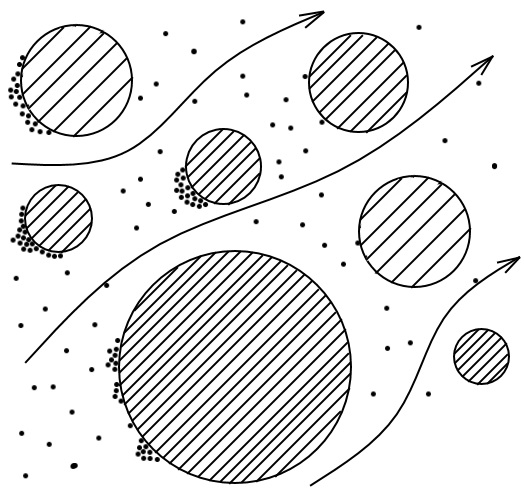
\includegraphics[width=7cm]{Particles_and_skeleton.jpg}}
\caption{Схема течения на уровне пор}
\label{fig:image1}
\end{figure}
\par Предполагается, что частицы имеют размер много меньше размера пор (во многих приложениях размер пор $d_{\text{ч}}\approx$ 1 мкм), перемещаются только благодаря потоку жидкости, перемешивание отсутствует. Это означает, что скорость частиц равна скорости жидкости. Также предполагается, что жидкость и частицы --- \textit{несжимаемые}, $\rho_{\text{ч}} = const, \; \rho_{\text{жидк}}\equiv\rho = const$.

\begin{figure}[h!]
\center{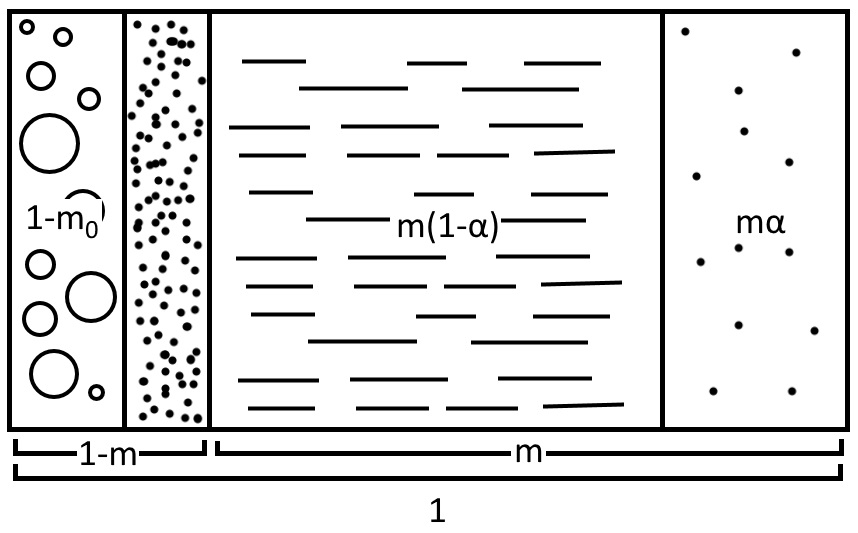
\includegraphics[width=10cm]{particles_quantity.jpg}}
\caption{Количество частиц в терминах $\alpha$ и $m$}
\label{fig:image2}
\end{figure}


\subsection{Законы сохранения массы}
\par Как и в других разделах механики сплошной среды, в теории фильтрации действуют стандартные законы сохранения. Их можно записать для каждой из фаз, для флюида и для частиц.
\par Запишем закон сохранения массы для жидкости:
$$\displaystyle \frac{d}{dt}\int\limits_{V}\rho m (1-\alpha)\,dV = - \int\limits_{\Sigma}\rho u_{n}(1-\alpha)\,d\sigma$$

\par Применяя стандартную технику перехода к дифференциальной форме, получим уравнение неразрывности для жидкой фракции:
$$
\begin{aligned}
\displaystyle 
\frac{\partial}{\partial t}(m(1-\alpha))+div((1-\alpha)\vec{u})=0
\end{aligned}
\eqno{(1)} 
$$
\par Также можно выписать соотношение на разрыве: 
$$[m(1-\alpha)]D-[(1-\alpha)u_{n}]=0$$
\par или в эквивалентной форме:
$$[m(\alpha-1)]D-[\alpha u_{n}]=0$$

\par Запишем аналогичный закон для частиц.

$$\displaystyle \frac{d}{dt}\int\limits_{V}{\rho_{\text{ч}}m\alpha+\rho_{\text{ч}}((1-m)-1-m_{0})}dV=-\int\limits_{\Sigma}\rho_{\text{ч}}\vec{u}\alpha d\sigma$$
\par Здесь $m_{0}=const$ --- первоначально пласт однородный. Перепишем полученные равенства в виде уравнения неразрывности:\\
$$(m\alpha)_{t}-m_{t}+div(\alpha \vec{u})=0$$
$$
\begin{aligned}
\displaystyle 
(m\alpha)_{t}+div(\alpha \vec{u})=m_{t}
\end{aligned}
\eqno{(2)} 
$$

\par Соотношение на разырыве:
$$[m\alpha-m]D-[\alpha u_{n}]=0$$

\par \textbf{Следствие:} Складывая (1)+(2) получаем уравнение неразрывности для \textbf{всей} суспензии.\\
$$m_{t}+div\;\vec{u}=m_{t}$$
$$div\;\vec{u}=0$$
\par Это уравнение можно использовать вместо (1) или (2) при решении системы уравнений.

\subsection{Закон Дарси}
\par В теории фильтрации используется экспериментальный закон Дарси, который связывает скорость и градиент давления. Этот закон можно получить как частное следствие закона Навье-Стокса при осреднении. Закон Дарси имеет вид:
$$
\begin{aligned}
\displaystyle 
-\vec{\nabla}P-\frac{\mu}{k}\vec{u}=0
\end{aligned}
\eqno{(3)} 
$$
\par В нашей постановке полагается, что массовых сил нет. В данной работе вязкость будет определяться в следующем виде:
$\mu=\mu(\alpha)=\mu_{0}(1+C\alpha)\approx\mu_{0},\;\;$
$k=k(m)$
\par В этой работе во многих задачах (3) отщепляется от системы.

\subsection{Кинетическое уравнение}

\par В исследуемой задаче функция, описывающая отложение частиц, считается известной, мы будем полагать, что данная зависимость имеет следующий вид:
$$
\begin{aligned}
\displaystyle 
m_{t}=-f(|\vec{u}|, m, \alpha)
\end{aligned}
\eqno{(4)} 
$$

\par С учётом кинетического уравнения мы можем выписать полную систему уравнений для поставленной задачи.

$$\displaystyle \begin {cases}
(m\alpha)'_{t}+(\alpha u)'_{x}=m'_{t}\\
u'_{x}=0\\
\displaystyle -P'_{x}-\frac{\mu}{k}u=0\\
m_{t}=-f(|\vec{u}|, m, \alpha)\\
\end {cases}$$

\subsection{Классификация системы уравнений}
\par В системе 6 уравнений и 6 неизвестных, $m, \alpha, P, \vec{u}$\\
\par Выписав систему уравнений для одномерных течений, можно получить матрицы с коэффициентами при производных переменных по $t$ (матрица $A_{ij}$) и по $x$ ($a_{ij}$). Если при этом у характеристического уравнения $|A_{ij}x-a_{ij}|=0$ все корни действительные, то система гиперболическая. Из этого следует, что уравнения в системе в характеристическом виде содержат производные по одному направлению (для каждого уравнения). Для нашей системы:\\
\bigskip
\\
$
\begin{cases}
\begin{aligned}
&(m\alpha)'_{t}+(\alpha u_{0})'_{x}=m'_{t}\\
&m_{t}=-f(|\vec{u}|, m, \alpha)
\end{aligned}
\end{cases}$
$\Leftrightarrow$
$
\begin{cases}
\begin{aligned}
&m\alpha'_{t}+\alpha m'_{t}+u_{0}\alpha'_{x}=m'_{t}\\
&m_{t}=-f(|\vec{u}|, m, \alpha)
\end{aligned}
\end{cases}$\\
\medskip
$\\
\begin{cases}
\begin{aligned}
&m\alpha'_{t}+(\alpha-1) m'_{t}+u_{0}\alpha'_{x}=0\\
&m_{t}=-f(|\vec{u}|, m, \alpha)
\end{aligned}
\end{cases}$
$\Leftrightarrow$
$
\begin{cases}
\begin{aligned}
&m\alpha'_{t}+u_{0}\alpha'_{x}=(\alpha-1)f(|\vec{u}|, m, \alpha)\\
&m_{t}=-f(|\vec{u}|, m, \alpha)
\end{aligned}
\end{cases}$\\
\bigskip
\\
\par Можно разделить производные (в каждом уравнении производные вдоль своего направления), значит система гиперболическая.